\begin{figure}[htb]
    \centering
    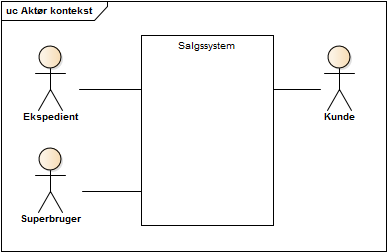
\includegraphics[width=0.5\textwidth]{Kravspecifikation/Billeder/Aktorcont.PNG}
    \caption{Aktør kontekst diagram for salgssystemet.}
    \label{fig:aktcont}
\end{figure}

Det ses hvordan både \gls{Eks} og \gls{SB} er de primære aktører for systemet.
På baggrund af aktør kontekstdiagrammet i figur \ref{fig:aktcont}, er følgende aktørbeskrivelse udarbejdet.


\begin{table}[H]
    \begin{tabularx}{\textwidth}{|l|X|}
\hline
	\textbf{Navn} & Ekspedient \\
\hline
 	\textbf{Type} & Primær \\
\hline
	\textbf{Beskrivelse} & \gls{Eks} er en primær bruger af systemet, som benytter systemet til at sælge og returnere varer. \\
\hline
\end{tabularx}
\captionsetup{justification=raggedright,singlelinecheck=false}
\caption{Aktør beskrivelse af \gls{Eks}}
\label{tab:AktEks}
\end{table}

\begin{table}[H]
    \begin{tabularx}{\textwidth}{|l|X|}
\hline
	\textbf{Navn} & \gls{SB} \\
\hline
 	\textbf{Type} & Primær \\
\hline
	\textbf{Beskrivelse} & \gls{SB} er en primær bruger af systemet, som benytter systemet til at oprette, nedlægge og redigere i systemets varekatalog. \\
\hline
\end{tabularx}
\captionsetup{justification=raggedright,singlelinecheck=false}
\caption{Aktør beskrivelse af \gls{SB}}
\label{tab:AktSuu}
\end{table}

\begin{table}[H]
    \begin{tabularx}{\textwidth}{|l|X|}
\hline
	\textbf{Navn} & Kunde \\
\hline
 	\textbf{Type} & Sekundær \\
\hline
	\textbf{Beskrivelse} & Kunden er en sekundær bruger af systemet, som ønsker at købe/returnere en eller flere varer igennem \gls{Eks}.   \\
\hline
\end{tabularx}
\captionsetup{justification=raggedright,singlelinecheck=false}
\caption{Aktør beskrivelse af kunden}
\label{tab:AktKu}
\end{table}


\newpage
